\documentclass[12pt, letterpaper]{article}

% Paquetes de idioma y tipografía
\usepackage[utf8]{inputenc}
\usepackage[T1]{fontenc}
\usepackage[spanish]{babel}
\usepackage{helvet}

% Configuración de márgenes
\usepackage[top=3.5cm, bottom=2.5cm, left=2.5cm, right=2.5cm, headheight=40pt]{geometry}

% Gráficos (El parámetro 'demo' dibuja cajas negras. QUITAR 'demo' al compilar con tus propias imágenes)
\usepackage{graphicx}


\begin{document}
\graphicspath{{images/}}

\vspace*{1.5cm}

\begin{center}
    % Reemplaza 'logo_centro.png' con tu archivo para el logo grande
    
\includegraphics[width=6.5cm, height=9cm]{images/logo.png}

    \vspace{2cm}

    {\Huge PPS \par}

    \vspace{2.5cm}

    {\large Estudiante: Eric Alexander Szuka \par}
    \vspace{0.8cm}
    {\large Docente: Carlos G. Lopez Pombo \par}
    
\end{center}

\newpage

\section{Introduccion}
  Para establecer los conocimientos obtenidos durante el recorrido de la carrera, el estudiante debe someterse a una actividad practica que requiera la implementacion de dichos conocimientos ya se mediante su insercion al mercado laboral, el desarrollo de una tesis o la incorporacion a un proyecto tanto de investigacion o de produccion ya existente. Este documento trata con el ultimo caso, en el cual se le permitio al estudiante incorporarse al proyecto RT-Constellation bajo la tutela del docente Carlos G. Lopez Pombo.

  La incorporacion del estudiante se basa en el hecho de que existe un problema el cual el estudiante es capaz de resolver, siendo este problema el hacer una reingenieria de una herramienta ya desarrollada y funcional, para que la herramienta sea mas acorde a su objetivo de ser una herramienta modular. 
  
 Actualmente la herramienta funciona de la siguiente forma, se estructura como una arquitectura descentralizada (por eso se define como una constelacion) diseñada para aislar la ejecucion del Sistema Bajo Prueba (SUT) de las tareas de verificacion. El objetivo de este diseño es evitar que el proceso de analisis, el cual requiere un alto nivel de procesamiento computacional, se convierta en algo que modifique el tiempo de ejecucion del SUT. Para lograrlo, el procesos se divide en agentes independientes que se comunican segun el tipo de rol que tengan (productor o consumidor) a travez de una infraestructura de paso de mensajes construida con RabbitMQ. 

 El ciclo de ejecucion de la herramienta esta centrado sobre 2 herramientas:
 \begin{itemize}
  \item \emph{Event reporter}:
    Este agente se encarga de dirigir la ejecucion del SUT en un hilo independiente, adquiriendo los datos en tiempo de ejecucion para producir un un flujo de eventos que es enviado a un canal de comunicacion llamado Event exchange
  \item \emph{Runtime Monitor}:
    Este agente actua como consumidor conectacal al Event exchange y se encarga de implementar el analisis logico leyendo y decodificando los eventos entrantes segun su clasificacion. Durante el procesamiento de eventos, el monitor verifica si la ejecucion cumple con las restricciones estructurales esperadas y utiliza un modulo evaluados de propiedades para confirmar su validez. Aparte de esto, el agente gestiona un diccionario con "gemelos digitales" para simular logicamente y hacer un seguimiento del estado de los componentes internos del SUT que no son visibles al proceso de verificacion
 \end{itemize}
 Luego de que los eventos sean evaluados existe un proceso de salida e interpretacion de resultados que consiste en lo siguiente:
 \begin{enumerate}
  \item El \emph{Runtime Monitor} produce un veredicto sobre cada propiedad analizada y emite estos resultados hacia un nuevo canal de RabbitMQ llamado \emph{Analysis results exchange}. En caso de detectar una falla, la herramienta tambien reporta la especificacion que sirve como evidencia del error.
  \item Diferentes agentes se encargan de leer esta informacion resultante de forma paralela para resumirla y/o procesarla.
  \item El agente Results Logger lee los resultados del intercambio y genera un reporte detallado en un archivo CSV.
  \item El agente \emph{Analysis stats} recopila las estadisticas durante el analisis, cuantificando propiedades fallidas o exitosas, y reportando la traza de eventos particular que ha sido ejecutada.
  \item Por ultimo, la herramienta tambien provee mecanismos para poder reejecutar analisis de forma identica; para esto cuenta con el agente \emph{Event writer}, el cual permite registrar los eventos emitidos inicialmente en un archivo, y el agente \emph{Event reader}, que permite volver a inyectar estos eventos leidos desde el archivo hacia el Event exchange.
 \end{enumerate}

\begin{figure}[htbp]
  \centering
  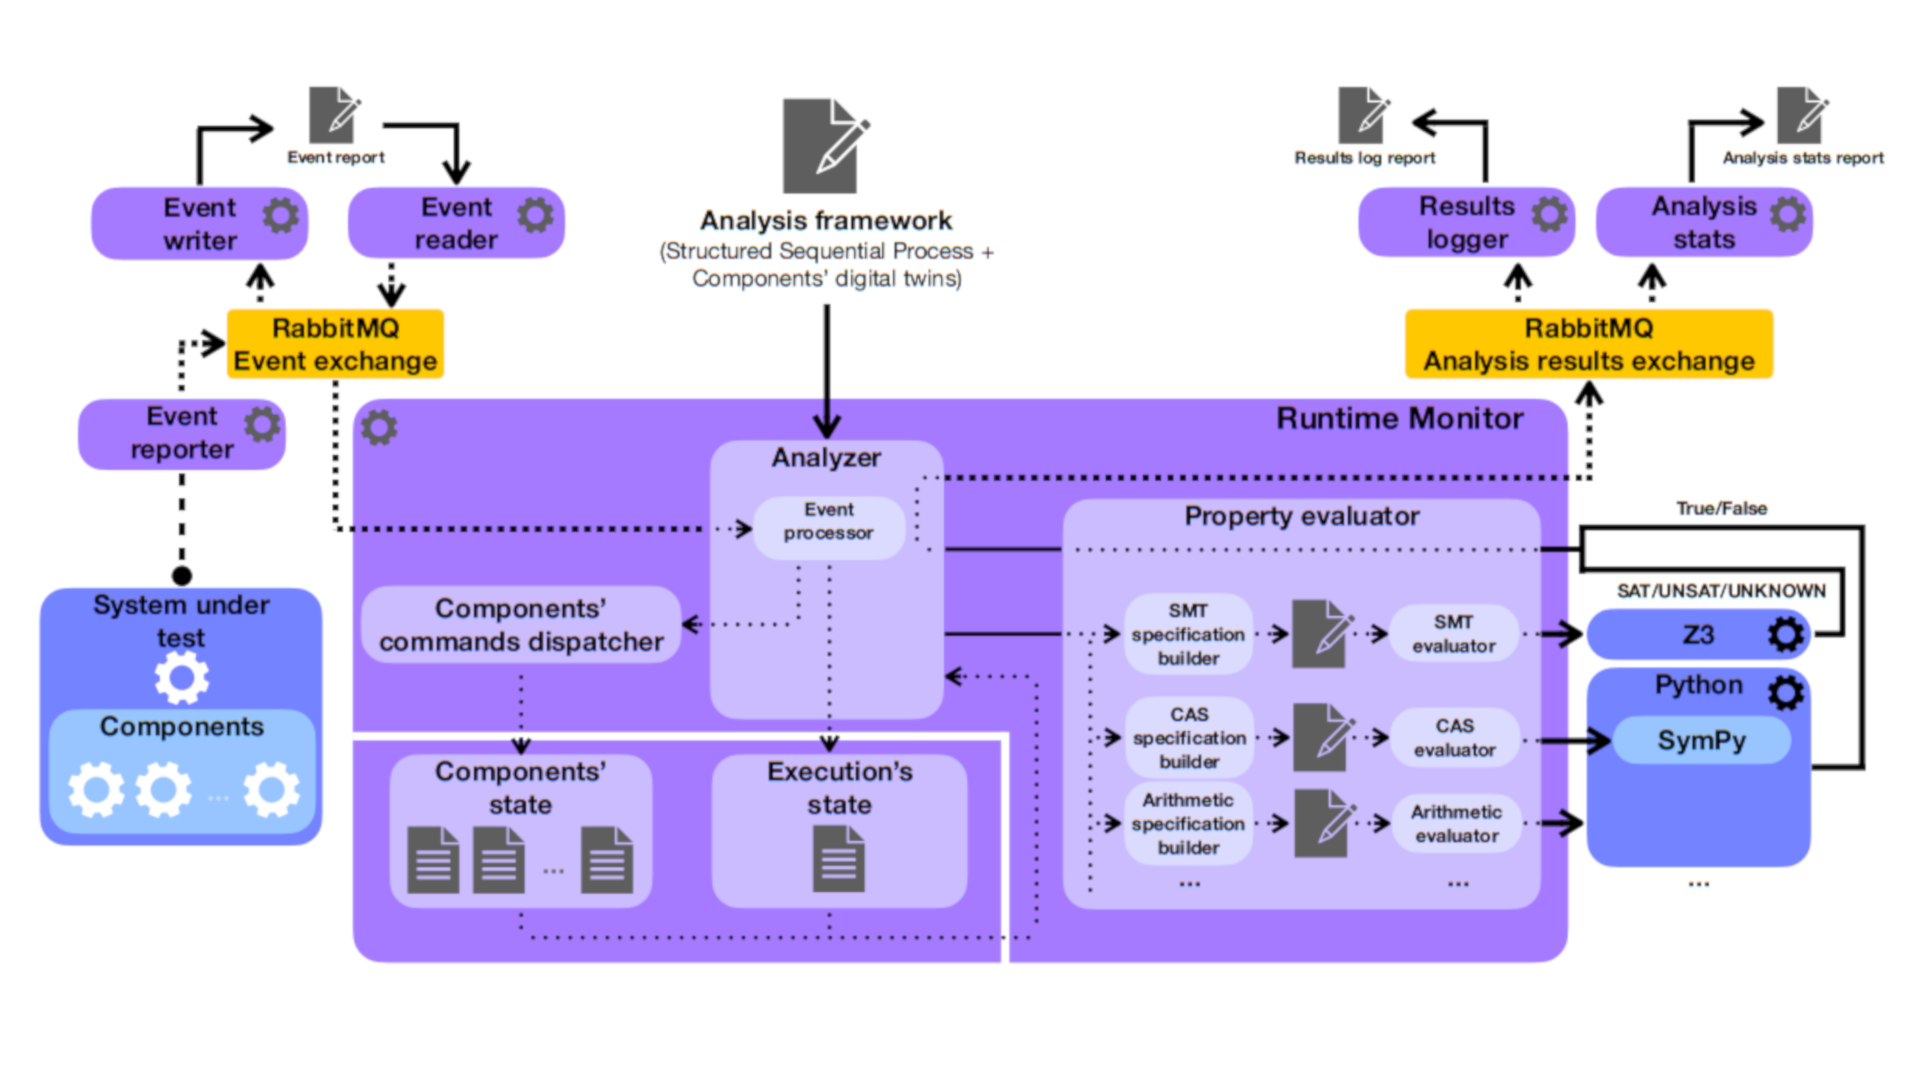
\includegraphics{rt-constellation-workflow}
  \caption{Workflow del RT-Constellation.}
  \label{fig:mi_etiqueta}
\end{figure}
  
  Esta forma de trabajar que tiene la herramienta funciona y permite su ejecucion exitosa, pero tiene un problema cuando se debe terminar su ejecucion y es que actualmente lo que sucede cuando el monitor termina su ejecucion al encontrarse con una propiedad erronea, este envia un mensajes de terminacion denominados \emph{poison pill} solamente a los agentes que tienen un rol de consumidor en los canales con un rol de productor, dejando en un estado de ejecucion permanente aquellos agentes que tienen un rol de productor en los canales que tienen rol de consumidor.
  
  Debido a esto, el docente le propuso al estudiante la siguiente solucion: Hacer una reingenieria de la constelacion para que incluya canales de control que permita que los agentes se comuniquen entre si para dar respuesta a este tipo de interacciones independientemente del rol que cumplan en la infraestructura.
\end{document}

